\documentclass[conference]{IEEEtran}
\IEEEoverridecommandlockouts
\usepackage{cite}
\usepackage{amsmath,amssymb}
\usepackage{graphicx}
\usepackage{booktabs}
\usepackage{url}
\usepackage{xurl}
\usepackage[hidelinks]{hyperref}

\newcommand{\code}[1]{\texttt{#1}}

\begin{document}

\title{Silent Updates: In-Place Revisions of Hugging Face Models Change What Deployed Classifiers Predict}

\author{\IEEEauthorblockN{Nitin Sarvesh S R}
\IEEEauthorblockA{\textit{Department of Computer Science} \\
\textit{CHRIST (Deemed to be University)}\\
Bengaluru, India \\
nitinsarvesh360@gmail.com}}

\maketitle

\begin{abstract}
Code usually loads a model from the Hugging Face Hub by name, and a name is not a version: the owner can replace the weights, label map or tokenizer in the same repository, and every user who has not pinned a revision receives it silently. We measure how often this happens, what it does to predictions, and whether it helps. For the 962 most downloaded text-classification models, we rebuild each commit history from git metadata and compare the release state with the current state on identical inputs. Of 875 models with loadable weights, 280 (32.0\%) differ in a file affecting inference, but most differences are automated format conversions that change nothing. Predictions changed for 53 of 62 models whose checkpoint was genuinely rewritten (85.5\%) and for none of 154 whose change was a conversion or metadata edit, so counting changed files overstates behavioural change roughly twofold. Rewriting affects 11.4\% of these models and 12.5\% of 1,499 further models across six other task types. Risk is front-loaded: 77.3\% are unchanged after a year. Re-evaluating 20 changed models on gold-labelled data shows the direction is unpredictable: six improved and two degraded significantly before multiple-comparison correction, the worst by 12.1 accuracy points on a model downloaded 142,000 times a month. One prompt-injection filter showed no significant accuracy change while the share of attacks it missed rose from 25.3\% to 51.3\%. Almost nobody pins: none of 1,783 Hub Spaces and 1.9\% of 7,720 GitHub code fragments do. We release the data and scripts.
\end{abstract}

\begin{IEEEkeywords}
software supply chain, pre-trained models, Hugging Face, model versioning, reproducibility
\end{IEEEkeywords}

\section{Introduction}

Pre-trained models are now ordinary software dependencies. The PeaTMOSS dataset alone maps more than 15,000 GitHub repositories to the Hub models they use \cite{peatmoss}, and the usual way to use one is a single call to the \code{transformers} library \cite{wolf2020}:

\begin{center}
\code{pipeline("text-classification", model="org/model")}
\end{center}

A package index such as PyPI does not allow a published file name to be reused with different content \cite{pypi-reuse}. A Hub model repository works differently. It is a git repository, and a model name without a revision resolves to the head of its \code{main} branch \cite{hf-repos}. When the owner commits new weights, the same line of code starts loading a different model. Banyongrakkul et al.\ found that only 12\% of GitHub projects that reuse Hub models specify a revision at all \cite{banyongrakkul2026}. The remaining 88\% track whatever the owner last pushed.

Whether this matters depends on something nobody has measured: when a popular model changes after release, how different are its predictions, and is the new version better? Earlier studies count commits, compare version names or read the metrics that owners report in model cards \cite{castano2024,ajibode2024,jia2025}. None of them runs the old and new versions of a model on the same inputs. That distinction decides the answer. A commit that adds a \code{safetensors} copy of existing weights and a commit that retrains the model are both ``the weight files changed'', and we find the first kind is the more common one and never changes a prediction.

Our results do not support the intuitive claim that silent updates degrade models: on each model's own task, updates improved accuracy more often than they hurt it. The problem is narrower. The change is unannounced, its direction is unpredictable, and the metrics a careful user would check can stay flat while the error profile moves: a prompt-injection guard in our sample kept its accuracy and doubled the share of attacks it admits.

We ask five research questions.
\begin{itemize}
\item \textbf{RQ1 (prevalence).} How often do popular models change files that affect inference after their initial release?
\item \textbf{RQ2 (impact).} When they change, how much do predictions change, and does the change alter labels, label names or the label space?
\item \textbf{RQ3 (detectability).} Which signals available without a GPU predict a behavioural change?
\item \textbf{RQ4 (exposure).} Do downstream applications on the Hub pin model revisions, and were they built before the model changed?
\item \textbf{RQ5 (direction).} On the model's own task, does the current version do better or worse than the released one?
\end{itemize}

We contribute a method separating a format conversion from a genuine rewrite using git metadata alone; a behavioural measurement of in-place updates across the top 962 text classifiers; a gold-labelled re-evaluation of their direction; a measurement of pinning in Hub Spaces and public GitHub code; and an open dataset with scripts that reproduce every number on a free GPU.

\section{Background and Related Work}

\subsection{How the Hub resolves a model name}
Every model on the Hub is a git repository whose large files are stored with Git LFS \cite{hf-repos}. \code{from\_pretrained} accepts an optional \code{revision} argument: a branch, a tag or a 40-character commit hash. Without it the library requests the files of \code{main} and, when online, downloads anything that changed, so a local cache does not protect a user from updates. Pinning a commit hash is the only way to guarantee the same bytes everywhere, and the Bandit security linter already reports unpinned downloads as issue B615 \cite{bandit-b615}.

\subsection{Model evolution and reuse on the Hub}
Jiang et al.\ reported that missing version information makes model reuse harder \cite{jiang2023}, and PeaTMOSS links GitHub projects to the models they load \cite{peatmoss}. Castaño et al.\ mined the commit histories of more than 380,000 Hub models and classified their maintenance activity \cite{castano2024}; Ajibode et al.\ found 148 different release-naming practices and concluded version numbers are often arbitrary \cite{ajibode2024}; Jia et al.\ tracked owner-reported metrics across versions \cite{jia2025}; Kadasi et al.\ re-evaluated 500 sentiment models and found reported performance often does not hold \cite{kadasi2025}; and Banyongrakkul et al.\ found low rates of revision pinning downstream \cite{banyongrakkul2026}. These studies describe the metadata of updates; we measure their effect on outputs.

\subsection{Backward compatibility of model updates}
Bansal et al.\ showed that a more accurate update can still hurt users who had learned the old behaviour \cite{bansal2019}, Srivastava et al.\ measured backward compatibility across retraining scenarios \cite{srivastava2020}, and Yan et al.\ named inputs an update gets wrong after the old model got them right \emph{negative flips} \cite{yan2021}. All assume the deploying team chose the update. On the Hub someone else chooses it and the user may not know, and a repository has no enforced versions at all.

\section{Method}

\subsection{Sample}
We listed the most downloaded models with the \code{text-classification} pipeline tag on 1 October 2026, excluding test repositories and exported ONNX, GGUF and OpenVINO copies, which left 962 models. Text classification is a good starting point because the output is a discrete label, so a change is easy to define, and because these models are often used as gates in larger systems: toxicity, prompt injection, spam and hate-speech filters.

\subsection{Rebuilding the history}
For each model we make a bare, blob-less git clone, which downloads commits and file trees but no weights. From \code{git log --raw} we replay every commit and track three groups of files that change inference: the weights \code{transformers} loads (\code{model.safetensors} or \code{pytorch\_model.bin} at the repository root, including shards); \code{config.json}, which holds the label map; and tokenizer files. When both weight formats are present we follow the library and treat the \code{safetensors} file as the loaded one. Files such as \code{training\_args.bin} are ignored, because they change on every training run but never reach a user. Git LFS pointer blobs change exactly when the stored file changes, so the history is exact without downloading any weights. All 962 repositories took about 40 minutes and no GPU, so we also applied it to six further pipeline tags.

\subsection{Release state and latest state}
Many repositories are created by a training script that pushes a checkpoint every epoch, so the first upload is often not the released model. Let $t_0$ be the time of the first commit containing loadable weights. The \emph{release state} $R$ is the last state at or before $t_0 + 7$ days; the \emph{latest state} $L$ is the head of \code{main} on the collection date. Section~\ref{sec:grace} reports other grace periods.

\subsection{Classifying a change}\label{sec:kinds}
We divide weight changes into three kinds, because they have different causes and different consequences.

\begin{itemize}
\item \textbf{Rewritten in place.} The effective weight file has the same format at $R$ and $L$ but different content: new parameters were written over the old ones.
\item \textbf{Pure format conversion.} The effective format changed from \code{.bin} to \code{.safetensors} while the original \code{.bin} stayed byte-identical. This is the signature of the Hub's conversion bot, which adds a second copy of the same weights that the library then prefers.
\item \textbf{Rewrite with format switch.} The format changed \emph{and} the \code{.bin} also changed, so the new file is not a conversion of the published checkpoint.
\end{itemize}

Tracking the \code{.bin} history separately is what makes this separation possible, and it is free, since it also comes from LFS pointer blobs.

\subsection{Behavioural comparison}
We load $R$ and $L$ at their exact commit hashes and run both on the same inputs: the 872 sentences of the SST-2 validation set \cite{socher2013} and 2,000 sentences from a multilingual language-identification corpus \cite{papluca}, 100 in each of 20 languages, since many models in the sample are not English. We compare outputs, not accuracy, and record the \emph{index flip rate} (share of inputs whose predicted class index differs, which is what code using the class index sees), the \emph{name flip rate} (share whose predicted label string differs), whether the number of classes changed, and the mean absolute change in the top-class probability.

Runs use \code{transformers} 4.57.6 on an NVIDIA T4, in fp32, batches of 32, inputs truncated to 128 tokens, and never execute repository code (\code{trust\_remote\_code=False}). Some release configs omit the model type or label count; we copy only the missing field from the latest config and flag the model. If a classification head is missing from either checkpoint the library initialises it randomly, so any flip would be noise; we detect this from the loading report and exclude those models.

\subsection{Gold-labelled re-evaluation}\label{sec:gold}
A flip rate on generic sentences does not say whether the update is an improvement. We therefore re-ran 21 models, 20 of them changed, spanning prompt-injection guards, toxicity and NSFW filters, and multilingual and financial sentiment, on gold-labelled data from their own task and language. We report accuracy, macro F1, an exact McNemar test on paired correctness, and for binary safety models the share of attacks missed and the false-positive rate.

Label names may have been renamed between versions, so we never assume an index order. For each version independently we search every mapping from its classes onto the gold classes, require the mapping to use every gold class, and keep the one that maximises that version's own accuracy. Each version is therefore scored at its best possible orientation, and a measured drop cannot be an artefact of renaming. As a pipeline check we included three models that RQ2 found behaviourally unchanged: one whose weights never changed and two whose files differ but which relabelled nothing.

\subsection{Downstream Spaces}
For every changed model we list up to 50 public Spaces declaring it as a dependency, read up to eight Python files from each, and check whether the model name appears. A use counts as pinned if a \code{revision} argument or a 40-character hash appears within three lines of the name. Creation and last-modified times tell us whether a Space predates the change. Because Spaces are largely demonstrations, we repeat the question with GitHub code search for every changed model and an equal-sized seeded sample of unchanged ones, applying the same pinning test. GitHub indexes only default branches, so counts are lower bounds.

\subsection{Statistics}
Proportions carry 95\% Wilson score intervals \cite{wilson1927}. Where noted, shares are weighted by monthly downloads at collection time as a proxy for exposure.

\section{Results}

\subsection{RQ1: How often do models change after release?}
We retrieved histories for 945 of the 962 models; 875 contain loadable weights, and the rest publish only adapters, remote code or non-standard files. Of these, 222 (25.4\%) have different effective weight files at $L$ than at $R$, 149 changed \code{config.json}, 85 changed tokenizer files, and 280 (32.0\%) differ in at least one. The release definition shifts this figure in the expected direction but not the conclusion: grace periods of 1, 30 and 90 days give weight-change rates of 30.9\%, 21.8\% and 16.3\%, so even discarding every update in the first quarter after publication, one model in six has different weights today.\label{sec:grace}

Splitting by the kinds of Section~\ref{sec:kinds} changes the picture (Table~\ref{tab:prev}). More than half of the weight changes (122 of 222) are pure format conversions by the Hub's bot. Only 100 models (11.4\%, CI [9.5, 13.7]) had their stored checkpoint genuinely rewritten; those repositories serve about 2.5 million downloads a month.

The changes are not announced. Of 834 post-release weight-change commits, 618 (74.1\%, CI [71.0, 77.0]) do not touch \code{README.md} in the same commit, so the model card describes a model that is no longer there. The median gap between release and first weight change is 117 days and the 90th percentile is 867 days, so these are not early post-release fixes. An older version is rarely left reachable: only 5 of the 222 changed models (2.3\%, CI [1.0, 5.2]) have any tag or branch besides \code{main}.

\textbf{The risk is front-loaded.} Treating the first post-release rewrite as an event and the collection date as a censoring time, a Kaplan--Meier estimate over all 875 models gives a survival rate of 80.3\% at 180 days, 77.3\% at one year and 76.3\% at both two and three years. The curve is flat after the first year: a model not rewritten within a year of release almost never is. Pinning therefore buys most during a model's first year.

Two properties do \emph{not} predict a rewrite. Popularity does not: rates by download quartile are 11.4\%, 16.5\%, 9.6\% and 8.2\%, the pattern is not monotonic, a Cochran--Armitage trend test gives $p = 0.086$, and top against bottom quartile gives $p = 0.335$, so a user cannot treat a popular model as a stable one. Age does not either ($r = -0.05$, $p = 0.15$). Safety classifiers are no exception: 14.4\% of 125 guards, filters and detectors were rewritten against 10.9\% of the other 750, with overlapping intervals.

\begin{table}[t]
\caption{Changes between release state and latest state (875 models with loadable weights)}
\label{tab:prev}
\centering
\footnotesize
\begin{tabular}{lrr}
\toprule
 & Models & Share \\
\midrule
Effective weight files differ & 222 & 25.4\% \\
\code{config.json} differs & 149 & 17.0\% \\
Tokenizer files differ & 85 & 9.7\% \\
Any inference-relevant file differs & 280 & 32.0\% \\
\midrule
\multicolumn{3}{l}{\emph{by kind of change}} \\
Rewritten in place (same format) & 82 & 9.4\% \\
Rewrite with format switch & 18 & 2.1\% \\
Pure format conversion (bot) & 122 & 13.9\% \\
Config or tokenizer only & 58 & 6.6\% \\
Unchanged since release & 595 & 68.0\% \\
\midrule
\textbf{Checkpoint genuinely rewritten} & \textbf{100} & \textbf{11.4\%} \\
\bottomrule
\end{tabular}
\end{table}

\textbf{The pattern is not specific to text classification.} We repeated the history stage, which needs no GPU, on the 250 most downloaded models of six further pipeline tags (Table~\ref{tab:tags}). Across all 1,499 models with loadable weights, 188 (12.5\%, CI [11.0, 14.3]) had their checkpoint rewritten, close to the 11.4\% of the main sample. The text-classification row is an independent draw from the same tag at a shallower depth and gives 8.6\%, which does not differ significantly from the main study's 11.4\% (Fisher $p = 0.24$). The rate does vary strongly by modality ($\chi^2 = 74.4$, $p = 5\times10^{-14}$), from 1.6\% for token classification to 24.4\% for speech recognition, so a practitioner's exposure depends on what they build with. Only 85 of 250 object-detection repositories publish weights in a format \code{transformers} loads, since many ship other formats, so that row rests on a smaller base.

\begin{table}[t]
\caption{Checkpoint rewriting across pipeline tags, top 250 models each}
\label{tab:tags}
\centering
\footnotesize
\begin{tabular}{lrrr}
\toprule
Pipeline tag & $n$ & Rewritten & Any change \\
\midrule
Automatic speech recognition & 209 & 51 (24.4\%) & 46.4\% \\
Object detection & 85 & 16 (18.8\%) & 51.8\% \\
Sentence similarity & 238 & 40 (16.8\%) & 55.9\% \\
Fill-mask & 235 & 39 (16.6\%) & 70.2\% \\
Text classification & 233 & 20 (8.6\%) & 38.6\% \\
Image classification & 249 & 18 (7.2\%) & 53.4\% \\
Token classification & 250 & 4 (1.6\%) & 6.8\% \\
\midrule
\textbf{All seven tags} & \textbf{1,499} & \textbf{188 (12.5\%)} & \\
\bottomrule
\end{tabular}
\end{table}

\subsection{RQ2: How much do predictions change?}\label{sec:rq2}
We attempted the 261 changed models under 1.5\,GB and evaluated 216. Of the rest, 31 could not be loaded without repository code or tokenizer packages, 8 had a randomly initialised head, and 6 changed the number of output classes, which breaks the comparison and the user's code alike.

Across all 216, 53 models (24.5\%, CI [19.3, 30.7]) relabel at least one input, 35 (16.2\%) more than 10\%, and 10 (4.6\%) more than half. The aggregate hides the structure (Fig.~\ref{fig:flip}, Table~\ref{tab:kind}): among models rewritten in the same format, 43 of 46 relabel something and 28 relabel more than 10\%, with a median flip rate of 17\%, while among the 154 models whose change was a conversion or a config or tokenizer edit, not one relabelled a single input out of 2,872. Combining the rewrite kinds, a genuine rewrite changes predictions for 53 of 62 models (85.5\%, CI [74.7, 92.2]) against 0 of 154 (0.0\%, CI [0.0, 2.4]); Fisher's exact test gives $p = 1.7\times10^{-41}$.

\begin{figure}[t]
\centering
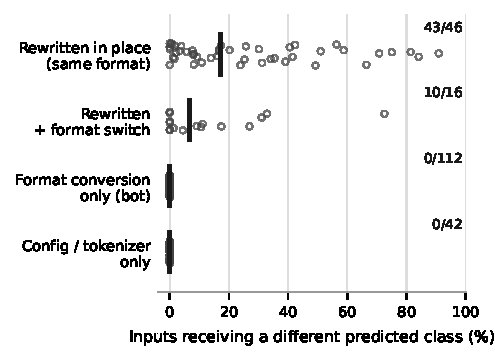
\includegraphics[width=\columnwidth]{fig_flip_by_kind.pdf}
\caption{Share of inputs receiving a different predicted class, by kind of repository change. Each circle is one model and the vertical bar is the group median; the fraction at the right of each row is the number of models with any changed prediction. Behavioural change is confined to models whose stored checkpoint was rewritten.}
\label{fig:flip}
\end{figure}

\begin{table}[t]
\caption{Behavioural effect by kind of change (216 evaluated models)}
\label{tab:kind}
\centering
\footnotesize
\begin{tabular}{lrrrr}
\toprule
Kind of change & $n$ & Any flip & $>10\%$ & Median \\
\midrule
Rewritten in place & 46 & 43 (93.5\%) & 28 & 17.0\% \\
Rewrite + format switch & 16 & 10 (62.5\%) & 7 & 6.8\% \\
Pure format conversion & 112 & 0 (0.0\%) & 0 & 0.0\% \\
Config or tokenizer only & 42 & 0 (0.0\%) & 0 & 0.0\% \\
\bottomrule
\end{tabular}
\end{table}

Three kinds of breakage follow, affecting different code. The first is behavioural: \path{MilaNLProc/feel-it-italian-sentiment} relabels 90.9\% of our inputs, and \path{tabularisai/multilingual-sentiment-analysis}, at about 157,000 downloads a month, relabels 51.0\%. The second is a change in names only: 27 models (12.5\%) return the same class index for every input but a different string, for example replacing \code{LABEL\_0} with a descriptive name, so a string test silently stops matching while every index-based test passes. The third is a change in the label space, where downstream code fails outright; six models did this, one with about 399,000 monthly downloads.

\subsection{RQ3: Which signals predict a behavioural change?}
The 0-of-154 result in Section~\ref{sec:rq2} is partly definitional: \code{safetensors} is a bit-exact serialisation, so a correct conversion \emph{should} preserve behaviour, and we confirm that it does. What follows is a correction to how the ecosystem is measured. A changed weight hash is a weak signal: of 174 evaluated models whose effective weight files differ, 121 (69.5\%, CI [62.3, 75.9]) give identical predictions on all 2,872 inputs, so a hash-based alarm is false about seven times in ten, and prevalence figures that count changed files overstate behavioural change by roughly a factor of two in our sample. The useful signal is narrower and just as cheap: asking whether the stored checkpoint was rewritten, by comparing the \code{.bin} history against the effective-format history, gives 53 true positives among 62 flagged models. Both need one blob-less clone and no GPU. No model changed behaviour through its config or tokenizer alone (0 of 42), although renaming still breaks string comparisons.

\subsection{RQ4: Are downstream applications protected?}
On the Hub, the 280 changed models are declared by 2,133 public Spaces, the model name appears in the Python source of 1,783, and \textbf{none} pins a revision (0 of 1,783, CI [0.0, 0.2]). Spaces are mostly demonstrations, though: only 101 were running at collection time, so we repeated the question against ordinary software.

Using GitHub code search we queried all 280 changed models and a matched random sample of 280 unchanged ones (560 queries, no failures). Public Python code names 69 of the 100 rewritten models, and the results we read, at most 30 per model, reference at least 754 distinct repositories depending on a rewritten checkpoint. Changed models are not less likely to have dependents than unchanged ones (239 of 280 against 223 of 280, Fisher $p = 0.095$), so this exposure is a property of the ecosystem rather than of which models change.

Pinning is almost as rare on GitHub as on the Hub: 143 of 7,720 matched code fragments pin a revision, 1.9\% (CI [1.6, 2.2]), and users of rewritten models are no better protected than users of unchanged ones (2.6\% against 2.5\%). Roughly 98\% of real projects that load these models take whatever is on \code{main}.

\subsection{RQ5: Does the update help or hurt?}\label{sec:rq5}
The 21 models were chosen because a public gold-labelled dataset exists for their task and language, which is a convenience sample rather than a random one: models with standard public benchmarks in their domain may be more conventionally maintained than the average changed model, so the proportions below describe this sample and not the population. Of the 21, 20 ran; one binary model could not be mapped onto a three-class gold set. Two more sit within 3 points of chance on the pooled data and one is multi-label, which our mapping does not support, leaving 17 usable comparisons.

Updates improved accuracy more often than they hurt it. Eight of the 17 changes are significant at $p<0.05$: six improvements and two degradations. Because this is 17 tests, we also apply a Holm--Bonferroni correction; six remain significant, four improvements and both degradations. The mean change is $+3.1$ points and the median $+0.9$. The largest gain, \path{UMUTeam/roberta-spanish-sentiment-analysis} at $+43.6$ points, comes from a release checkpoint scoring 35.9\% on a three-class task, below chance, which the update evidently repaired; it is a real fix rather than a typical case.

The two significant regressions are consequential. \path{StephanAkkerman/FinTwitBERT-sentiment}, about 142,000 downloads a month, falls from 95.1\% to 83.1\% on financial tweet sentiment ($p = 1.1\times10^{-32}$): 185 inputs the release version classified correctly are now wrong, against 28 the other way. \path{pysentimiento/robertuito-sentiment-analysis}, about 788,000 downloads a month, falls from 81.6\% to 76.9\% ($p = 9.2\times10^{-5}$).

A single case shows that accuracy can hide the change entirely. Table~\ref{tab:guards} gives the error profile of the prompt-injection guards that moved. \path{NeuralTrust/prompt-guard-oss-small} shows no significant accuracy change ($-0.9$ points, $p = 0.43$), yet the share of attacks it admits rises from 25.3\% to 51.3\% while its false-positive rate falls from 13.0\% to 0.5\%: the update moved the operating point towards permissiveness. This is one model, so we draw no rate from it; what it establishes is that the failure mode exists and that the metrics a careful user would check do not reveal it. For a sentiment model that trade is unremarkable; for a security filter it is the only thing that matters. Both \code{wolf-defender} guards moved the same way by smaller amounts; the two remaining guards were stable on both measures.

\begin{table}[t]
\caption{Prompt-injection guards: accuracy against error profile. Miss = attacks classified benign.}
\label{tab:guards}
\centering
\footnotesize
\begin{tabular}{lrrr}
\toprule
Guard & Accuracy & Miss rate & False pos. \\
\midrule
prompt-guard-oss-small & 82.7 $\to$ 81.8 & 25.3 $\to$ \textbf{51.3} & 13.0 $\to$ 0.5 \\
wolf-defender & 95.5 $\to$ 97.1 & 5.2 $\to$ 7.1 & 4.2 $\to$ 0.7 \\
wolf-defender-small & 95.9 $\to$ 95.9 & 7.1 $\to$ 10.2 & 2.6 $\to$ 0.8 \\
\bottomrule
\end{tabular}
\end{table}

\section{Discussion}

\textbf{For users.} Pin a revision. \code{from\_pretrained("org/model", revision="<40-hex commit>")} is a one-line change and Bandit already flags its absence as B615 \cite{bandit-b615}. Pair the pin with a deliberate, tested upgrade, since a pinned model never receives a fix either and six of our eight significant changes were improvements. The test should compare predictions on a fixed input set, and for a classifier that gates something it must look at the error profile, not the aggregate: our clearest example kept its accuracy and doubled its miss rate.

Pinning costs little: of 705 rewrite commits classified by message, 3.1\% claim an explicit fix, 58.9\% describe a retrain or improvement and 38.0\% say nothing informative, so a pinned user forgoes mostly undocumented retraining, and the exposure removed is concentrated in a model's first year.

\textbf{For model owners.} Treat a published model as immutable. Retrain into a new repository, or at least tag the old commit, which only 2.3\% of owners who overwrote weights did. If weights are overwritten, say so in the model card: three quarters of the changes we saw did not touch the README. Renaming labels deserves equal care, since it breaks string comparisons while leaving every accuracy metric intact.

\textbf{For the Hub.} Its own conversion bot produces exactly the change we found never alters behaviour. An alert on every weight-file change would be mostly noise; one on a checkpoint rewrite would be specific and cheap. Two mechanisms would help most: an immutable release marker, as package indexes forbid reusing a file name \cite{pypi-reuse}, and a notification to watchers and dependent Spaces when a checkpoint is rewritten.

\section{Threats to Validity}\label{sec:threats}

\textbf{Construct.} Our release state is a heuristic; a repository whose real release came long after its first weights is judged against too early a baseline, and Section~\ref{sec:grace} bounds this. The gold sets in Section~\ref{sec:gold} are proxies for each model's deployment distribution, so the direction we measure is the direction on a public benchmark of the same task. Granting each version its best label mapping is generous to both and may slightly overstate the accuracy of a model whose label semantics we cannot recover.

\textbf{Internal.} Our RQ2 inputs are generic sentences rather than each model's domain, but the magnitude is stable: the 872 SST-2 sentences alone give a median flip rate of 18.8\% against 17.4\% on all 2,872 ($r = 0.87$ across models), and only 3 of 216 models differ by more than 25 points, all with a language or task the English inputs do not match. We have no noise floor, since we do not know how much two legitimately equivalent checkpoints would differ, so a small flip rate is not evidence of a meaningful change. Excluding the 16 models that needed a repaired config or fallback tokenizer changes nothing. Three models that RQ2 found unchanged also showed exactly zero disagreement in RQ5 on different data, which argues that the pipeline does not manufacture differences. The rewrite-versus-conversion label comes from file history, not commit messages, and the two agree for 212 of 222 changed models (95.5\%); the rest were both converted and, separately, rewritten. RQ5 covers 17 models, which supports the existence and shape of both outcomes but no precise population rate. Some of the 1,783 Space matches are comments or interface text rather than a live load, which overstates usage but not the pinning result, since a pin would appear next to the name wherever the model is loaded.

\textbf{External.} Behavioural measurements cover text classifiers only; the multi-tag scan extends the prevalence result to six other tags but not the prediction comparison. Generative models deserve separate study. Every number is a measurement of 1 October 2026, and the Hub keeps moving.

\section{Conclusion}
A model name on the Hugging Face Hub does not identify a fixed model. About one in three of the most downloaded text classifiers has changed a file that affects inference since release, but most of those changes are automated conversions that provably leave predictions alone. About one in nine had its checkpoint rewritten in place, a rate that holds across six other pipeline tags, and predictions changed for 85\% of those. The direction is not uniform harm but unannounced and unpredictable change: two of seventeen models got significantly worse, one by 12 points with six-figure monthly downloads, and a prompt-injection guard doubled the share of attacks it admits while its accuracy stood still. Almost no downstream code pins a revision: none of 1,783 Space files and 1.9\% of 7,720 GitHub fragments, while at least 754 GitHub repositories depend on a rewritten model. Pinning is a one-line fix, telling a rewrite from a conversion is cheap enough to monitor, and the larger fix is for model hubs to make released versions immutable, as package indexes have long done. Our dataset and scripts are available at \url{https://github.com/nitin30-git/silent-updates} and archived at \url{https://doi.org/10.5281/zenodo.23157456}.

\section*{Acknowledgment}
The author used an AI assistant (Claude, Anthropic) to help write the data collection and analysis code and to draft and edit parts of this manuscript. The author designed the study, ran all experiments, checked the results against the raw data and is responsible for the content.

\begin{thebibliography}{00}
\bibitem{peatmoss} W. Jiang, J. Yasmin, J. Jones, N. Synovic, J. Kuo, N. Bielanski, Y. Tian, G. K. Thiruvathukal, and J. C. Davis, ``PeaTMOSS: A dataset and initial analysis of pre-trained models in open-source software,'' in \textit{Proc. 21st Int. Conf. Mining Software Repositories (MSR)}, 2024.
\bibitem{wolf2020} T. Wolf \textit{et al.}, ``Transformers: State-of-the-art natural language processing,'' in \textit{Proc. EMNLP: System Demonstrations}, 2020, pp. 38--45.
\bibitem{pypi-reuse} Python Package Index, ``Why am I getting a `this filename has already been used' error?'' PyPI Help. [Online]. Available: \url{https://pypi.org/help/#file-name-reuse}
\bibitem{hf-repos} Hugging Face, ``Repositories,'' Hugging Face Hub documentation. [Online]. Available: \url{https://huggingface.co/docs/hub/repositories}
\bibitem{banyongrakkul2026} P. Banyongrakkul, M. Zahedi, C. Treude, H. Gao, and P. Thongtanunam, ``When AI models become dependencies: Studying the evolution of pre-trained model reuse in downstream software systems,'' arXiv:2604.17940, 2026.
\bibitem{castano2024} J. Castaño, S. Martínez-Fernández, X. Franch, and J. Bogner, ``Analyzing the evolution and maintenance of ML models on Hugging Face,'' in \textit{Proc. 21st Int. Conf. Mining Software Repositories (MSR)}, 2024.
\bibitem{ajibode2024} A. Ajibode, A. A. Bangash, F. R. Cogo, B. Adams, and A. E. Hassan, ``Towards semantic versioning of open pre-trained language model releases on Hugging Face,'' arXiv:2409.10472, 2024.
\bibitem{jia2025} N. Jia, A. Raja, and R. Khatchadourian, ``An empirical framework for evaluating semantic preservation using Hugging Face,'' arXiv:2512.07983, 2025.
\bibitem{bandit-b615} PyCQA, ``B615: huggingface\_unsafe\_download,'' Bandit documentation. [Online]. Available: \url{https://bandit.readthedocs.io/en/latest/plugins/b615_huggingface_unsafe_download.html}
\bibitem{jiang2023} W. Jiang \textit{et al.}, ``An empirical study of pre-trained model reuse in the Hugging Face deep learning model registry,'' in \textit{Proc. 45th Int. Conf. Software Engineering (ICSE)}, 2023.
\bibitem{kadasi2025} P. Kadasi \textit{et al.}, ``Model hubs and beyond: Analyzing model popularity, performance, and documentation,'' in \textit{Proc. Int. AAAI Conf. Web and Social Media (ICWSM)}, vol. 19, no. 1, 2025, pp. 965--993.
\bibitem{bansal2019} G. Bansal, B. Nushi, E. Kamar, D. S. Weld, W. S. Lasecki, and E. Horvitz, ``Updates in human-AI teams: Understanding and addressing the performance/compatibility tradeoff,'' in \textit{Proc. AAAI Conf. Artificial Intelligence}, 2019.
\bibitem{srivastava2020} M. Srivastava, B. Nushi, E. Kamar, S. Shah, and E. Horvitz, ``An empirical analysis of backward compatibility in machine learning systems,'' in \textit{Proc. 26th ACM SIGKDD Int. Conf. Knowledge Discovery and Data Mining (KDD)}, 2020.
\bibitem{yan2021} S. Yan \textit{et al.}, ``Positive-congruent training: Towards regression-free model updates,'' in \textit{Proc. IEEE/CVF Conf. Computer Vision and Pattern Recognition (CVPR)}, 2021.
\bibitem{socher2013} R. Socher \textit{et al.}, ``Recursive deep models for semantic compositionality over a sentiment treebank,'' in \textit{Proc. EMNLP}, 2013, pp. 1631--1642.
\bibitem{papluca} papluca, ``language-identification,'' Hugging Face dataset. [Online]. Available: \url{https://huggingface.co/datasets/papluca/language-identification}
\bibitem{wilson1927} E. B. Wilson, ``Probable inference, the law of succession, and statistical inference,'' \textit{J. Amer. Statist. Assoc.}, vol. 22, no. 158, pp. 209--212, 1927.
\end{thebibliography}

\end{document}
